\documentclass[aspectratio=169]{beamer}
\usepackage{generic}
\begin{document}

\begin{frame}
  \title{\darkblue Introduction to the TAF package\\[1ex]
    \normalsize\darkgreen 3~ TAF features}
  \author{\vspace{-16ex}\small\darkgray\it Arni Magnusson and Colin Millar}
  \date{}
  \titlepage
\end{frame}

% ______________________________________________________________________________

\begin{frame}{Overview}
  \begin{itemize}
    \item[] {\bf\darkblue 1~ Background} \comment{objectives, design}\\[3ex]
    \item[] {\bf\darkblue 2~ Running a TAF analysis} \comment{linear regression,
      boot and run, structured scripts}\\[3ex]
    \item[] {\bf\darkblue 3~ TAF features} \comment{boot procedure, data flow,
      new analysis, overview of functions}\\[3ex]
    \item[] {\bf\darkblue 4~ The TAF community} \comment{browsing an existing
      analysis, related R packages}\\[3ex]
    \item[] {\bf\darkblue 5~ Discussion} \comment{contents of a TAF analysis,
      benefits of TAF}\\[3ex]
    \item[] {\bf\darkblue 6~ Online examples} \comment{ICES, FAO, SPC,
      various}\\[3ex]
  \end{itemize}
\end{frame}

% ______________________________________________________________________________

\begin{frame}{The boot procedure}\small
  \begin{itemize}
    \item[] Similar to booting a computer, the TAF boot procedure readies the
    data and\\[0.2ex]
    software components that are required for subsequent computations.\\[4ex]
    \item[] The boot procedure takes place inside the boot folder, where the
    {\tt\blue taf.boot()}\\[0.2ex]
    function looks for files called {\darkgreen DATA.bib} (required) and
    {\darkgreen SOFTWARE.bib} (optional).\\[4ex]
    \item[] In the {\tt linreg} example, the DATA.bib file contains a single
    metadata entry:\\[2ex]\tt\fns
    {\darkgray @Misc}\{ezekiel.txt,\\
    ~ {\green originator} = \{Mordecai Ezekiel\},\\
    ~ {\green year} ~~~~~ = \{1930\},\\
    ~ {\green title} ~~~~ = \{Speed of automobile and distance to stop after
    signal\},\\
    ~ {\green source} ~~~ = \{file\},\\
    \}\\[5ex]
  \end{itemize}
\end{frame}

% ______________________________________________________________________________

\begin{frame}{The boot procedure}\small
  \begin{itemize}
    \item[] The source field specifies where data or software originate from.
    The following\\[0.2ex]
    types of values can be used in the source field:\\[2ex]
    \begin{enumerate}
      \item {\green GitHub reference} of the form {\tt owner/repo[/subdir]@ref},
      identifying a\\
      specific version of a GitHub resource.\\[2ex]
      \item {\green URL}, identifying a file to download.\\[2ex]
      \item Special value {\tt\green script}, indicating that a boot script (a
      custom R script) should\\
      be run to fetch or produce files, e.g., by querying local or online
      databases.\\[2ex]
      \item {\green Relative path} starting with {\tt initial}, identifying the
      location of a file or\\
      directory somewhere inside the {\tt boot/initial} folder.\\[2ex]
      \item Special value {\green {\tt file} or {\tt folder}}, indicating that
      the file or folder is inside {\tt boot/initial/data} or
      {\tt boot/initial/software}.\\[5ex]
    \end{enumerate}
  \end{itemize}
\end{frame}

% ______________________________________________________________________________

\begin{frame}{The flow of data}\small
  \begin{itemize}
    \item[] There are several important differences between the
    {\tt boot/initial/data} folder\\[0.2ex]
    and the {\tt boot/data} folder:\\[1ex]
    \begin{itemize}
      \item[-] The {\tt\green boot/initial/data} folder is where the scientist
      can make initial\\
      data files available that are not coming from online data
      repositories.\\[2ex]
      \item[-] The {\tt\orange boot/data} folder is machine-generated and its
      contents should not\\
      be manually edited by the user. This folder will be regenerated and\\
      overwritten whenever the boot procedure is run.\\[2ex]
      \item[-] The contents of the {\tt\orange boot/data} folder are guaranteed
      to come with\\
      descriptive metadata that are declared in the {\tt DATA.bib} file. The
      purpose\\ of the metadata is to elevate the level of data quality and
      transparency.\\[2ex]
      \item[-] The {\tt data.R} script reads from the {\tt\orange boot/data}
      folder and not from {\tt\green boot/initial/data}.\\[4ex]
    \end{itemize}
  \end{itemize}
\end{frame}

% ______________________________________________________________________________

\begin{frame}{The flow of data}\small
  \vspace{1ex}
  \qquad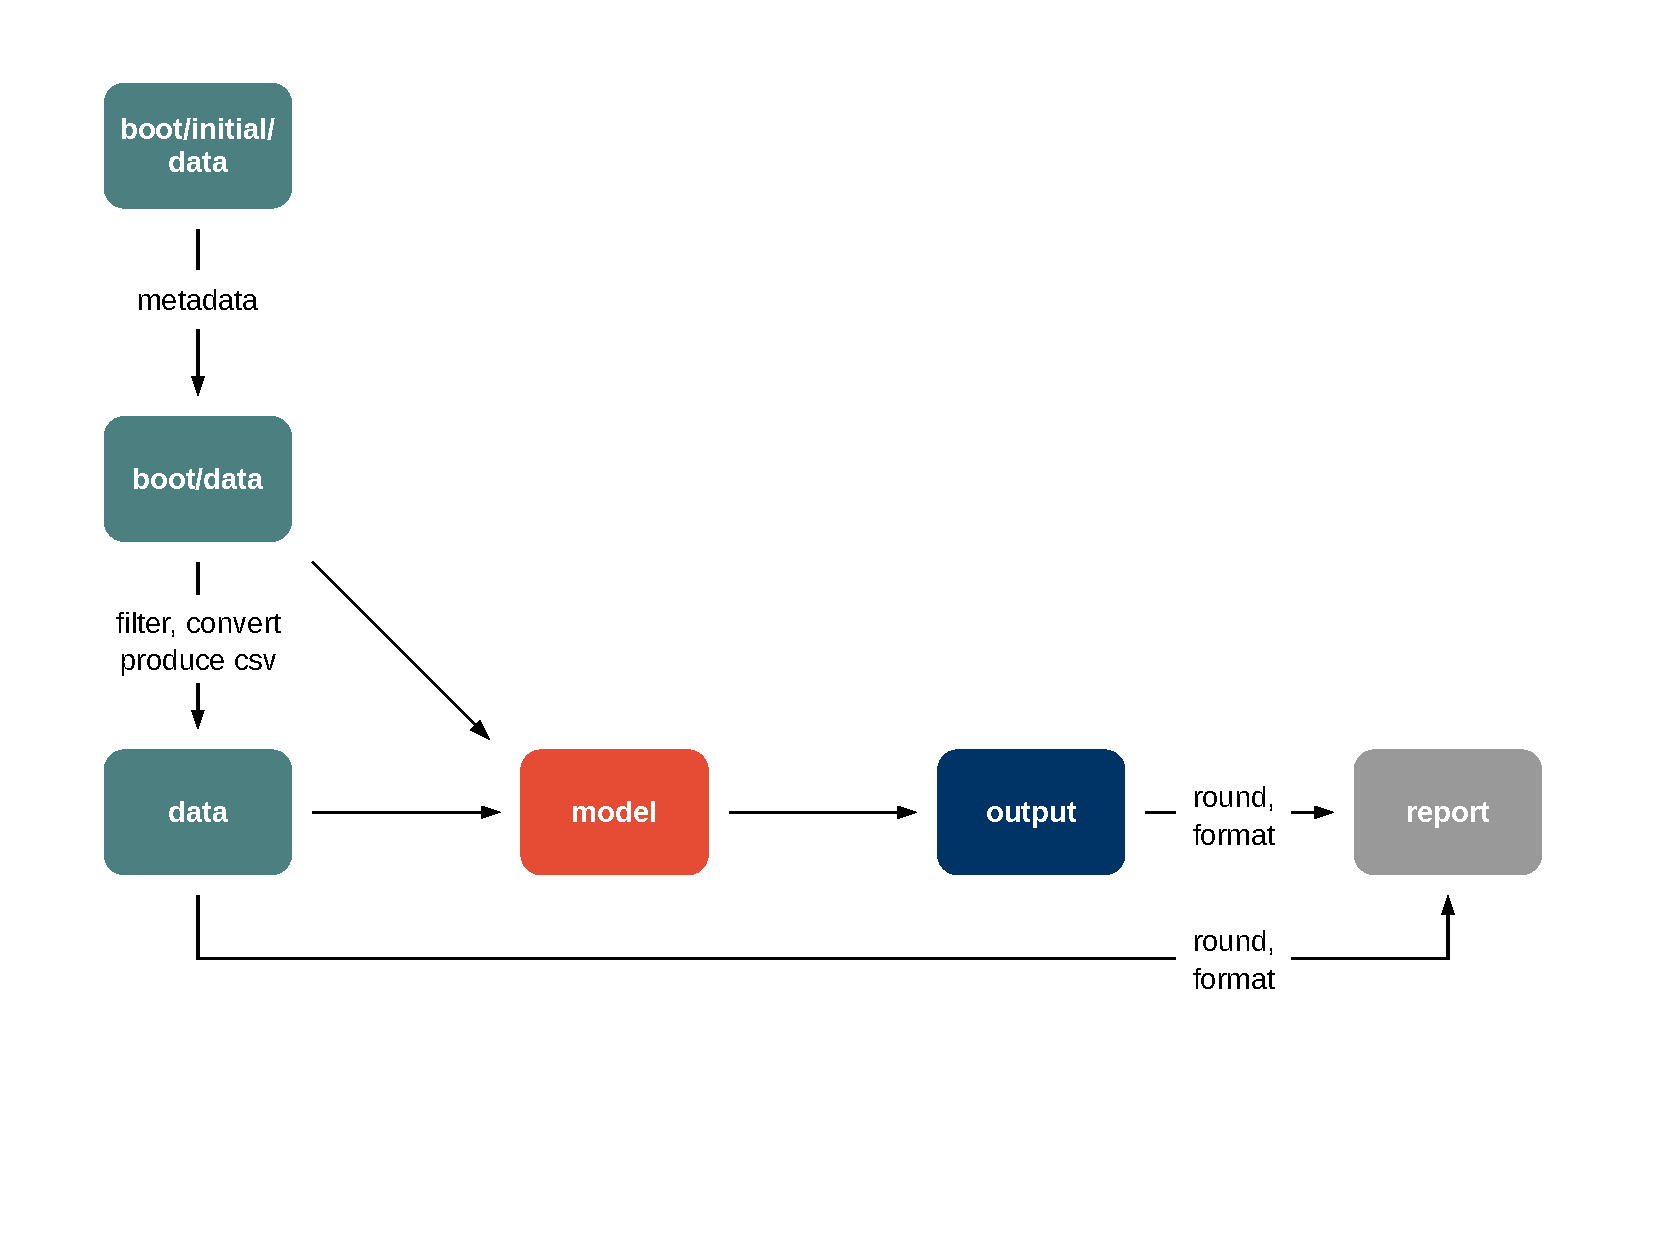
\includegraphics[width=0.75\textwidth]{data}
\end{frame}

% ______________________________________________________________________________

\begin{frame}{Creating a new analysis}\small
  \begin{itemize}
    \item[] When authoring a TAF analysis, one can either start with a new
    workflow or\\
    from a similar workflow and adapt it to the current analysis.\\[2ex]
    The {\tt\blue taf.skeleton()} function creates a new workflow, consisting of
    an empty\\
    {\tt boot/initial/data} folder and the four TAF scripts: {\tt data.R},
    {\tt model.R},\\
    {\tt output.R}, and {\tt report.R}.\\[2ex]
    Each script provides a starting point for that step of the analysis, for
    example,\\
    a new {\tt data.R} script contains the following lines:\\[2ex]\tt\fns
    {\gray \# Prepare data, write CSV data tables}\\[2ex]
    {\gray \# Before:}\\
    {\gray \# After:}\\[2ex]
    {\blue library}(TAF)\\[2ex]
    {\blue mkdir}("data")\\[4ex]
  \end{itemize}
\end{frame}

% ______________________________________________________________________________

\begin{frame}{Creating a new analysis}\small
  \begin{itemize}
    \item[] After running {\tt\blue taf.skeleton()} to create a new TAF
    workflow, the scientist\\[0.2ex]
    can populate the {\tt boot/initial/data} folder with initial data files and
    run\\[0.2ex]
    {\tt\blue draft.data(file=TRUE)} to produce a {\tt DATA.bib} file.\\[4ex]
    \item[] The next step is then to run {\tt\blue taf.boot()} to populate the
    {\tt boot/data} folder\\[0.2ex]
    and start editing the {\tt data.R} script.\\[6ex]
  \end{itemize}
\end{frame}

% ______________________________________________________________________________

\begin{frame}{Overview of functions}\small
  \begin{itemize}
    \item[] {\it Initial TAF steps}\\
    \begin{itemize}\tt\blue\fns
      \item[] draft.data
      \item[] draft.software
      \item[] taf.boot
      \item[] taf.example
      \item[] taf.skeleton\\[2ex]
    \end{itemize}
    \item[] {\it Running scripts}\\
    \begin{itemize}\tt\blue\fns
      \item[] source.all\\[2ex]
    \end{itemize}
    \item[] {\it File management}\\
    \begin{itemize}\tt\blue\fns
      \item[] mkdir
      \item[] read.taf
      \item[] write.taf\\[2ex]
    \end{itemize}
    \item[] {\it Plots}\\
    \begin{itemize}\tt\blue\fns
      \item[] taf.png\\[4ex]
    \end{itemize}
  \end{itemize}
\end{frame}

% ______________________________________________________________________________

\begin{frame}{Overview of functions}\small
  \begin{itemize}
    \item[] The TAF package provides many other functions that can be useful
    but\\[0.2ex]
    are not required for authoring or running TAF workflows.\\[4ex]
    \item[] Several TAF functions are designed to support running the same
    analysis\\[0.2ex]
    across different {\green operating systems} and {\green locales}, and every
    function comes\\[0.2ex]
    with a help page that includes {\green examples} and
    {\green cross-references}.\\[4ex]
    \item[] Furthermore, typing {\tt ?TAF} opens a {\green package help page}
    that gives an\\[0.2ex]
    overview of all the functions in the package, grouped by
    functionality.\\[6ex]
  \end{itemize}
\end{frame}

% ______________________________________________________________________________

\begin{frame}{Summary}
  \begin{itemize}
    \item[] {\bf\darkblue 1~ Background} \comment{objectives, design}\\[3ex]
    \item[] {\bf\darkblue 2~ Running a TAF analysis} \comment{linear regression,
      boot and run, structured scripts}\\[3ex]
    \item[] {\bf\darkblue 3~ TAF features} \comment{boot procedure, data flow,
      new analysis, overview of functions}\\[3ex]
    \item[] {\bf\darkblue 4~ The TAF community} \comment{browsing an existing
      analysis, related R packages}\\[3ex]
    \item[] {\bf\darkblue 5~ Discussion} \comment{contents of a TAF analysis,
      benefits of TAF}\\[3ex]
    \item[] {\bf\darkblue 6~ Online examples} \comment{ICES, FAO, SPC,
      various}\\[3ex]
  \end{itemize}
\end{frame}

\end{document}
